\documentclass[10pt]{extarticle}
\title{}
\author{}
\date{}
\usepackage[shortlabels]{enumitem}


%paper setup
\usepackage{geometry}
\geometry{letterpaper, portrait, margin=1in}
\usepackage{fancyhdr}
% sans serif font:
\usepackage{cmbright}
%symbols
\usepackage{amsmath}
\usepackage{bigints}
\usepackage{amssymb}
\usepackage{amsthm}
\usepackage{mathtools}
\usepackage{bbm}
\usepackage[hidelinks]{hyperref}
\usepackage{gensymb}
\usepackage{multirow,array}
\usepackage{multicol}

\newtheorem*{remark}{Remark}
\usepackage[T1]{fontenc}
\usepackage[utf8]{inputenc}

%chemistry stuff
%\usepackage[version=4]{mhchem}
%\usepackage{chemfig}

%plotting
\usepackage{pgfplots}
\usepackage{tikz}
\tikzset{middleweight/.style={pos = 0.5}}
%\tikzset{weight/.style={pos = 0.5, fill = white}}
%\tikzset{lateweight/.style={pos = 0.75, fill = white}}
%\tikzset{earlyweight/.style={pos = 0.25, fill=white}}

%\usepackage{natbib}

%graphics stuff
\usepackage{graphicx}
\graphicspath{ {./images/} }
\usepackage[style=numeric, backend=biber]{biblatex} % Use the numeric style for Vancouver
\addbibresource{the_bibliography.bib}
%code stuff
%when using minted, make sure to add the -shell-escape flag
%you can use lstlisting if you don't want to use minted
%\usepackage{minted}
%\usemintedstyle{pastie}
%\newminted[javacode]{java}{frame=lines,framesep=2mm,linenos=true,fontsize=\footnotesize,tabsize=3,autogobble,}
%\newminted[cppcode]{cpp}{frame=lines,framesep=2mm,linenos=true,fontsize=\footnotesize,tabsize=3,autogobble,}

%\usepackage{listings}
%\usepackage{color}
%\definecolor{dkgreen}{rgb}{0,0.6,0}
%\definecolor{gray}{rgb}{0.5,0.5,0.5}
%\definecolor{mauve}{rgb}{0.58,0,0.82}
%
%\lstset{frame=tb,
%	language=Java,
%	aboveskip=3mm,
%	belowskip=3mm,
%	showstringspaces=false,
%	columns=flexible,
%	basicstyle={\small\ttfamily},
%	numbers=none,
%	numberstyle=\tiny\color{gray},
%	keywordstyle=\color{blue},
%	commentstyle=\color{dkgreen},
%	stringstyle=\color{mauve},
%	breaklines=true,
%	breakatwhitespace=true,
%	tabsize=3
%}
% text + color boxes
\renewcommand{\mathbf}[1]{\mathbbm{#1}}
\usepackage[most]{tcolorbox}
\tcbuselibrary{breakable}
\tcbuselibrary{skins}
\newtcolorbox{problem}[1]{colback=white,enhanced,title={\small #1},
          attach boxed title to top center=
{yshift=-\tcboxedtitleheight/2},
boxed title style={size=small,colback=black!60!white}, sharp corners, breakable}
%including PDFs
%\usepackage{pdfpages}
\setlength{\parindent}{0pt}
\usepackage{cancel}
\pagestyle{fancy}
\fancyhf{}
\rhead{Avinash Iyer}
\lhead{Algebra II: Class Notes}
\newcommand{\card}{\text{card}}
\newcommand{\ran}{\text{ran}}
\newcommand{\N}{\mathbbm{N}}
\newcommand{\Q}{\mathbbm{Q}}
\newcommand{\Z}{\mathbbm{Z}}
\newcommand{\R}{\mathbbm{R}}
\newcommand{\C}{\mathbbm{C}}
\setcounter{secnumdepth}{0}
\begin{document}
  \section{Motivation and Introduction}%
  Main purpose of this course is to study Galois theory --- a field that arose in trying to study roots of polynomials.\\

  Consider $f(x) = ax^2 + bx + c$. If we want to find a general, closed-form expression for the roots of the function, we complete the square.
  \begin{align*}
    \text{roots} &= \frac{-b \pm \sqrt{b^2-4ac}}{2a}.
  \end{align*}
  We found these roots by by the coefficients, $\Q$, addition, subtraction, multiplication, division, and square root (raising to the $1/2$ power: see Math 310 notes, Page 104). Naturally, this leads us to ask whether we can do this for cubic polynomials with the same operations. Obviously, we have to change from $1/2$ power to the $1/3$ power, but Cardano showed that it was possible to solve a cubic and quartic equation using these traditional operations and radicals.\\

  Évariste Galois invented his theory to prove there is no such closed formula by radicals for any polynomial of degree $5$ or above.\\

  For example, $x^5 - x + 1$ does not have roots given by radicals.
  \subsection{Example: A Solvable Polynomial}%
  Consider the polynomial $f(x) = x^2 - 2$. We know that the roots of this polynomial are $\pm \sqrt{2}$. From this, we want to create a set $K(f)$ that satisfies the following rules:
  \begin{itemize}
    \item $\Q \subseteq K(f)$.
    \item $K(f)$ must contain the roots of $f$.
    \item $K(f)$ must be closed under the traditional operations: $+,-,\times,/$
    \item $K(f)$ must be the smallest field that satisfies the above three requirements.
  \end{itemize}
  \textbf{Claim:} $K(f) = \Q(\sqrt{2}) = \{a + b\sqrt{2}\mid a,b\in \Q\}$.
  \begin{itemize}
    \item $\Q\subseteq K(f)$, because we can set $b=0$.
    \item $\sqrt{2} = 0 + (1)(\sqrt{2})$, $-\sqrt{2} = 0 + (-1)(\sqrt{2})$
    \item Let $a+b\sqrt{2}$ and $c+d\sqrt{2}$ be elements of $K(f)$. Then,
      \begin{itemize}
        \item $(a+b\sqrt{2})\pm (c+d\sqrt{2}) = (a\pm c) + (b\pm d)\sqrt{2}$
        \item $(a+b\sqrt{2})(c+d\sqrt{2}) = (ac + 2bd) + (ad + bc)\sqrt{2}$
        \item Set $c+d\sqrt{2} \neq 0$
          \begin{align*}
            \frac{a+b\sqrt{2}}{c+d\sqrt{2}} &= \frac{(a+b\sqrt{2})(c-d\sqrt{2})}{c^2-2d^2}\\
                                            &= \frac{1}{c^2-2d^2}\left((ac-2bd) + (bc-ad)\sqrt{2}\right)\\
                                            &= \frac{ac-2bd}{c^2-2d^2} + \frac{bc-ad}{c^2-2d^2}\sqrt{2}
          \end{align*}
      \end{itemize}
    \item $K(f)$ is indeed the smallest set.
      \begin{itemize}
        \item Note that $K(f)$ is a $\Q$-vector space, with basis $\{1,\sqrt{2}\}$. Therefore, $\text{dim}_{\Q} K(f) = 2$. $K(f)$ is known as the ``splitting field'' of $f$.
      \end{itemize}
  \end{itemize}

  We want to consider a bijective function $\varphi: K(f)\rightarrow K(f)$ with the following properties:
  \begin{itemize}
    \item $\varphi(r) = r$ for every $r\in\Q$
    \item $\varphi(x+y) = \varphi(x) + \varphi(y)$
    \item $\varphi(xy) = \varphi(x)\varphi(y)$
  \end{itemize}
  We denote the collection of all such $\varphi$ as $\text{Aut}(K(f)/\Q)$. This is a group under the operation $\circ$ (composition). Specifically, we have
  \begin{align*}
    \varphi(a+b\sqrt{2}) &= \varphi(a) + \varphi(b)\varphi(\sqrt{2})\\
                         &= a + b\varphi(\sqrt{2}).
  \end{align*}
  Notice
  \begin{align*}
    \left(\varphi(\sqrt{2})\right)^2 - 2 &= \varphi \left(\left(\sqrt{2}\right)^2 - 2\right)\\
                            &= \varphi(0)\\
                            &= 0.
  \end{align*}
  Therefore, $\varphi(\sqrt{2}) = \pm \sqrt{2}$. Therefore, we have that the elements of $\text{Aut}(K(f)/\Q)$ as the following:
  \begin{align*}
    \varphi_0: a+b\sqrt{2} \mapsto a+b\sqrt{2}\\
    \varphi_1: a+b\sqrt{2} \mapsto a-b\sqrt{2}\\
    \varphi_1\circ\varphi_1 = \varphi_0\\
    \shortintertext{Thus,}
    \text{Aut}(K(f)/\Q) &= \{\varphi_0,\varphi_1\}\\
                        &\cong \Z/2\Z
  \end{align*}
  \subsection{Example: A Harder Polynomial}%
  Let $f(x) = (x^2-2)(x^2-3)$. Our roots are $\{\pm\sqrt{2},\pm\sqrt{3}\}$. We want to form $K(f)$ with the same properties. Let
  \begin{align*}
    K(f) &= \Q(\sqrt{2},\sqrt{3})\\
    &= \{a+b\sqrt{2}+c\sqrt{3}+d\sqrt{6}\mid a,b,c,d\in\Q\}.
  \end{align*}
  Just as with our previous example, $K(f)$ is a vector space over $\Q$, with basis $\{1,\sqrt{2},\sqrt{3},\sqrt{6}\}$, so $\text{dim}_{\Q}K(f) = 4$.\\

  Now, we want $\text{Aut}(K(f)/\Q)$. If $\varphi\in \text{Aut}(K(f)/\Q)$, then
  \begin{align*}
    \varphi(a+b\sqrt{2}+c\sqrt{3}+d\sqrt{6}) &= a+b\varphi(\sqrt{2}) + c\varphi(\sqrt{3}) + d\varphi(\sqrt{6})\\
                                             &= a+b\varphi(\sqrt{2}) + c\varphi(\sqrt{3}) + d\varphi(\sqrt{2})\varphi(\sqrt{3}).
  \end{align*}
  Thus, we need to know $\varphi(\sqrt{2})$ and $\varphi(\sqrt{3})$. So,
  \begin{align*}
    f(\varphi(\sqrt{2})) &= \left(\left(\varphi(\sqrt{2})\right)^2 - 2\right)\left(\left(\varphi(\sqrt{2})\right)^2-3\right)\\
                         &= 0\\
                         \shortintertext{and the same is the case with $\varphi(\sqrt{3})$. So,}
    \varphi(\sqrt{2}) &\in \{\pm\sqrt{2}, \pm\sqrt{3}\}\\
    \varphi(\sqrt{3}) &\in \{\pm\sqrt{2},\pm\sqrt{3}\}.\\
    \shortintertext{Suppose $\varphi(\sqrt{2}) = \sqrt{3}$. Then,}
    \left(\left(\varphi(\sqrt{2})\right)^2\right) &= (\sqrt{3}^2-1)\\
                                                  &= 0\\
                                                  &=\left(\varphi(2)-3\right)\\
                                                  &= -1.~\bot\\
                                                  \shortintertext{Thus,}
    \varphi(\sqrt{2}) &\in \{\pm\sqrt{2}\}\\
    \varphi(\sqrt{3}) &\in \{\pm\sqrt{3}\},\\
    \shortintertext{and we have the maps as:}
    \varphi_0&: \sqrt{2}\mapsto\sqrt{2},\sqrt{3}\mapsto\sqrt{3}\\
    \varphi_1&: \sqrt{2}\mapsto-\sqrt{2},\sqrt{3}\mapsto\sqrt{3}\\
    \varphi_2&: \sqrt{2}\mapsto\sqrt{2},\sqrt{3}\mapsto-\sqrt{3}\\
    \varphi_3&: \sqrt{2}\mapsto-\sqrt{2},\sqrt{3}\mapsto-\sqrt{3}\\
  \end{align*}
  %\begin{center}
  %  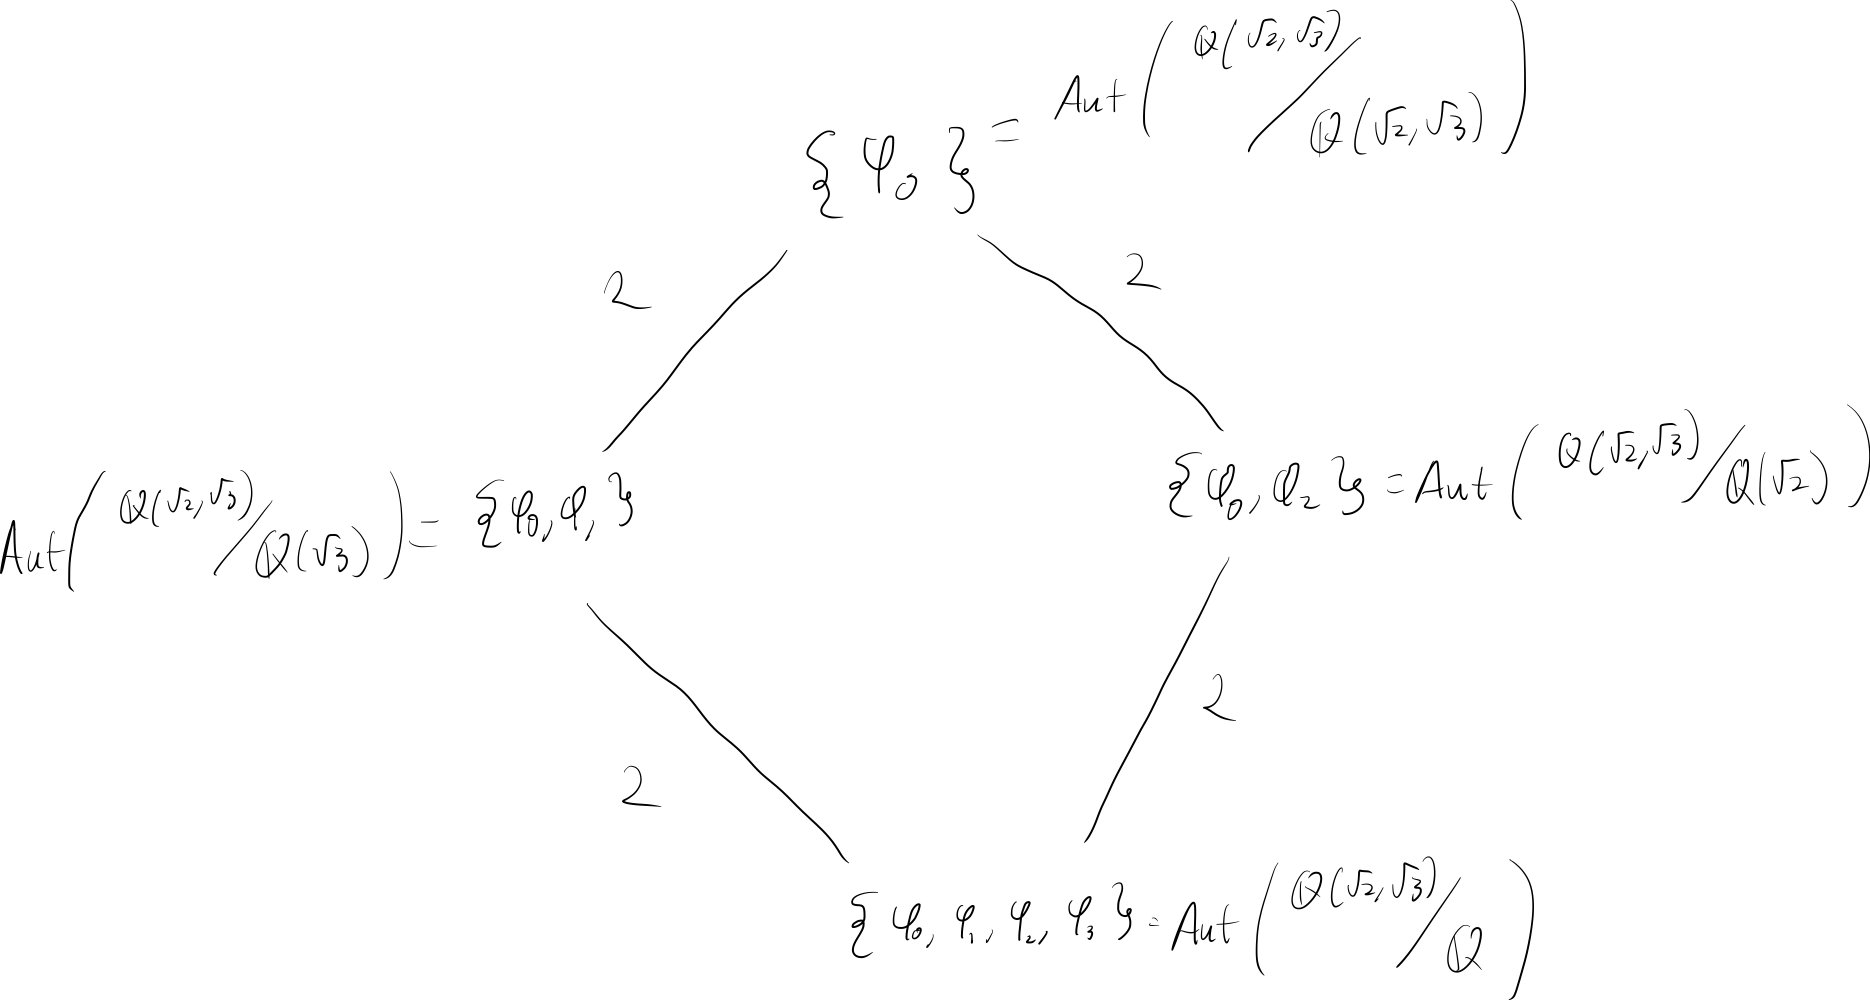
\includegraphics[width=\textwidth]{images/automorphism_lattice.png}
  %\end{center}
  % automorphism group lattice
  \subsection{Example: A Cubic Polynomial}%
  Consider the function $f(x) = x^3 - 2$. The function has one real root, $r_1=\sqrt[3]{2}$, and two complex roots. Let's examine $\Q(\sqrt[3]{2}) = \{a + b\sqrt[3]{2} + c\sqrt[3]{4}\mid a,b,c\in\Q\}$; $r_2$ and $r_3$ are not in $Q(\sqrt[3]{2})$. We could instead consider $\Q(\sqrt[3]{2},r_1,r_2)$.
  \begin{align*}
    x^3-2 &= (x-r_1)(x^2 + r_1x + r_1^2)\\
    r_2 &= \frac{-r_1 + \sqrt{r_1^2-4r_1^2}}{2}\\
        &= r_1\frac{-1+\sqrt{-3}}{2}\\
        &= r_1\zeta_3\\
    r_3 &= r_1\frac{-1 - \sqrt{-3}}{2}\\
        &= r_1\zeta_3^2
  \end{align*}
  However, including $r_2$ and $r_3$ is excessive --- all we need is $\Q(\sqrt[3]{2},\zeta_3)$. Therefore, the basis of this vector space is $\{1,r_1,r_1^2,\zeta_3,\zeta_3 r_1,\zeta_3 r_1^2\}$ (note that $\zeta_3^2 = -1-\zeta_3$). Therefore, $\text{dim}_{\Q}\Q(\sqrt[3]{2},\zeta_3)=6$, and $\Q(\sqrt[3]{2},\zeta_3) = K(f)$.Additionally, we have $\text{Aut}(\Q(\sqrt[3]{2})/\Q) = \{\varphi_0\}$, but $\dim_{\Q}\Q(\sqrt[3]{2}) = 3$. For the full field extension, we need to find $\varphi(\sqrt[3]{2})$ and $\varphi(\zeta_3)$.
  \begin{align*}
    \varphi(\sqrt[3]{2}) &\in \{r_1,\zeta_3 r_1,\zeta_3^2 r_1\}\\
    \varphi(\zeta) &\in \{\zeta_3,\zeta_3^2\}\\
    \varphi_0 &: r_1\mapsto r_1,\zeta_3\mapsto \zeta_3\\
    \varphi_1 &: r_1\mapsto \zeta_3r_1,\zeta_3\mapsto \zeta_3\\
    \varphi_2 &: r_1\mapsto r_1,\zeta_3\mapsto \zeta_3^2\\
    \varphi_3 &: r_1\mapsto \zeta_3^2r_1,\zeta_3\mapsto \zeta_3\\
    \varphi_4 &: r_1\mapsto \zeta_3r_1,\zeta_3\mapsto \zeta_3^2\\
    \varphi_5 &: r_1\mapsto \zeta_3^2r_1,\zeta_3\mapsto \zeta_3^2\\
    \shortintertext{Therefore,}
    \text{Aut}(\Q(\sqrt[3]{2},\zeta_3)/\Q) &= 6\\
                                           &= \dim_{\Q}\Q(\sqrt[3],\sqrt[3]{2})
  \end{align*}
  \section{Rings}%
  Consider the integers under the normal operations, $(\Z,+,\cdot)$; this will serve as the motivation for rings in the future.
  \subsection{Definition of a Ring}%
   Let $R$ be a nonempty set with operations $(+,\cdot)$, with the following properties:
    \begin{enumerate}[(1)]
      \item $(R,+)$ is an abelian group:
        \begin{itemize}
          \item Closed: $r_1 + r_2\in R,~ \forall r_1,r_2\in R$
          \item Identity: $\exists 0_R,~r + 0_R = 0_R+r = r$
          \item Associativity: $r_1 + (r_2 + r_3) = (r_1 + r_2) + r_3$
          \item Inverse: $\forall r\in R,~\exists -r\in R, r + (-r) = 0_R$
          \item Commutativity: $r_1 + r_2 = r_2 + r_1$
        \end{itemize}
      \item Closure under Multiplication: $r_1\cdot r_2\in R,~\forall r_1,r_2\in R$
      \item Associativity under Multiplication: $r_1\cdot (r_2 \cdot r_3) = (r_1\cdot r_2)\cdot r_3$
      \item Distributivity: $r_1\cdot (r_2 + r_3) = r_1\cdot r_2 + r_2\cdot r_3, (r_1 + r_2)\cdot r_3 = r_1\cdot r_3 + r_2\cdot r_3$
    \end{enumerate}
  We say $(R,+,\cdot)$ is a ring if it satisfies all these properties.\\

  If $\exists 1_R\in R$ such that $r\cdot 1_R = 1_R \cdot r = r$, then we say $R$ is a ring with identity, and $1_R$ is the multiplicative identity. If multiplication is commutative, then $R$ is known as a commutative ring.
  \subsubsection{Examples}%
  \begin{enumerate}[(1)]
    \item $(\Z,+,\cdot)$, $(\Q,+,\cdot)$, $(\R,+,\cdot)$, $(\mathbbm{C},+,\cdot)$ are commutative rings with identity value of $1$.
    \item $(\Z/n\Z,+,\cdot)$ is a commutative ring with identity $1_{R} = [1]_n$.
    \item $(\R[x],+,\cdot)$, where $\displaystyle\R[x] = \left\{\sum_{i=0}^{n}a_ix^i\mid a_i\in\R\right\}$, is a commutative ring with identity.
    \item $(2\Z,+,\cdot)$ is a commutative ring \textit{without} identity.
    \item $(\text{Mat}_{n}(\R),+,\cdot)$, where $\text{Mat}_n(\R)$ refers to $n\times n$ matrices with real entries, is a \textit{non}commutative ring with identity.
  \end{enumerate}
  \subsection{Division Rings and Fields}%
  Let $R$ be a ring with identity. We say $R$ is a \textit{division ring} if $\forall r\in R\setminus \{0_R\}$, $\exists r^{-1}\in R$ with $r\cdot r^{-1} = 1_R = r^{-1}\cdot r$. If $R$ is also commutative, then $R$ is a \textit{field}.
  \subsubsection{Examples}%
  \begin{enumerate}[(1)]
    \item $(\Q,+,\cdot)$, $(\R,+,\cdot)$, and $(\mathbbm{C},+,\cdot)$ are all fields.
    \item Let $p$ be prime, and set $F = \Z/p\Z$. Then, $F$ is a field; we denote this $\mathbbm{F}_p$.
    \item Define 
      \begin{align*}
        \mathbbm{H} = \{a+bi+cj+dk\mid a,b,c,d\in\R,i^2=j^2=k^2=-1,ij=k=-ji,jk=i=-kj,ki=j=-ik\}.
      \end{align*}
      Then, $\mathbbm{H}$ is a division ring, known as the Hamiltonian quaternions. Note that $\mathbbm{C}\subset \mathbbm{H}$.
  \end{enumerate}
  \subsection{Properties of Rings}%
  \begin{description}
    \item[Proposition 4.1:] Let $R$ be a ring.
      \begin{enumerate}[(1)]
        \item $0_R a = a0_r = 0$ $\forall a\in R$
        \item $(-a)b = a(-b) = -(ab)$ $\forall a,b\in R$
        \item $(-a)(-b) = ab$ $\forall a,b\in R$
        \item If $\exists 1_R\in R$, then $1_R$ is unique, and $-a = (-1_R)a$.
      \end{enumerate}
    \item[Proof of (1):] Let $a\in R$. Then,
      \begin{align*}
        0_Ra &= (0_R + 0_R)a \tag*{Additive Inverse}\\
        0_Ra &= 0_Ra + 0_Ra \tag*{Distributivity}\\
        0_Ra + (-0_Ra) &= 0_Ra + 0_Ra (-0_Ra)\\
        0_R &= 0_Ra. \tag*{Additive Inverse}
      \end{align*}
    \item[Proof of (2):] Let $a,b\in R$. Note that $-(ab)$ is the unique inverse such that $ab + (-(ab)) = 0_R$ via group theory. We have
      \begin{align*}
        ab + (-a)b &= (a+(-a))b \tag*{Distributivity}\\
                   &= (0_R)b\tag*{Additive Inverse}\\
                   &= 0_R. \tag*{By Property (1)}
      \end{align*}
      Thus, $(-a)b = -(ab)$.
  \end{description}
  \subsection{Zero Divisor and Units in Rings}%
    Let $a\in R$, $a\neq 0_R$. If $\exists b\in R$ with $b\neq 0_R$ such that $ab = 0_R = ba$, then we say $a$ is a zero divisor.\\

    If $1_R \in R$, we say $u\in R$ is a unit if $\exists v\in R$ (can be equal to $u$) with $uv = 1_R = vu$. The collection of units in $R$ is denoted $R^{\times}$.
    \begin{description}
      \tiny
      \item[Exercise:] Show that $R^{\times}$ is a group under multiplication.
    \end{description}
    \subsubsection{Examples}%
  \begin{enumerate}[(1)]
    \item Let $R = \Z/6\Z$. Note that $[2]_6 [3]_{6} = [6]_{6} = [0]_{6}$, so both $[2]_6$ and $[3]_{6}$ are both zero divisors. Additionally, $[4]_6[3]_6 = [6]_{6} = [0]_{6}$. Meanwhile, since $(\Z/6\Z)^{\times}=\{[1]_{6},[5]_{6}\}$, those are the two units of $\Z/6\Z$.
    \item $\Z$ has no zero divisors. $\Z^{\times} = \{\pm 1\}$.
    \item $\Q$ has no zero divisors. $\Q^{\times} = \Q\setminus \{0\}$.
    \item $\Z[i] = \{a+bi\mid a,b\in\Z,i^2=-1\}$ has no zero divisors (as $\mathbbm{C}$ is a field). $\Z[i]^{\times} = \{\pm 1,\pm i\}$.
  \end{enumerate}
  \subsection{Subrings}%
  Let $(R,+,\times)$. If $S\subseteq R$ is a nonempty subset, and $(S,+,\cdot)$ is a ring, then $S$ is a subring of $R$. To see $S$ is a subring, it is enough to show:
  \begin{itemize}
    \item $S\neq \emptyset$.
    \item $S$ is closed under subtraction.
    \item $S$ is closed under multiplication of elements in $S$.
  \end{itemize}
  \subsubsection{Examples}%
  \begin{enumerate}[(1)]
    \item 
    \begin{align*}
      \underbrace{\Z\subseteq\Q\subseteq\R\subseteq \mathbbm{C}}_{\text{subrings}}
    \end{align*}
  \item $\R\subseteq \R[x]$ is a subring.
  \item $S = \{[0]_4,[2]_4\}\subseteq \Z/4\Z$ is a subring.
  \end{enumerate}
  \subsection{Integral Domains}%
  Let $R$ be a commutative ring with identity. We say $R$ is an integral domain if $R$ has no zero divisors.
  \subsubsection{Examples}%
  \begin{enumerate}[(1)]
    \item $\Z$, the integers, is an integral domain, that is not a field.
    \item All fields are integral domains.
    \item $\Z/6\Z$ is \textit{not} an integral domain, as it has zero divisors.
    \item $\Z/n\Z$ is not an integral domain if $n$ is composite.
  \end{enumerate}
  Integral domains are nice due to allowance of cancellations. For example, if $2m = 2n$ in $\Z$, then we find $2(m-n) = 0$, and since $\Z$ has no zero divisors, it must be the case that $m=n$.\\

  However, in a ring that is not an integral domain, such as $\Z/6\Z$, we cannot use the same technique to find the solution to a similar equation. For example, $3\cdot 2 = 0 = 3\cdot 4$, but $2\neq 4$.
  \subsubsection{Proposition: Equations in Integral Domains}%
  Let $R$ be an integral domain. If $a,b,c\in R$ with $a\neq 0_R$, and $ab = ac$, then $b=c$.\\

  \textbf{Proof:}
  \begin{align*}
    ab &= ac\\
    a(b-c) &= 0_R\\
    \shortintertext{Since $a\neq 0$,}
    b-c &= 0_R\\
    b &= c.
  \end{align*}
  \subsubsection{Theorem: Finite Integral Domains and Fields}%
  If $R$ is an integral domain, and $\card(R) < \infty$ ,then $R$ is a field.\\

  \textbf{Proof:} Let $a\in R$, $a\neq 0_{R}$. Note $ab \neq 0_R$ for all $b\in R,~b\neq 0_R$.\\

  Define $\varphi_a: R\setminus\{0_R\} \rightarrow R\setminus\{0_R\}$, $b\mapsto ab$. If $\varphi_a(b) = \varphi_a(c)$, then $ab = ac$, and by our previous result, $b=c$ --- therefore, $\varphi_a$ is injective.\\

  Since $R\setminus \{0_R\}$ is finite, and $\varphi_a$ is injective, then $\varphi_a$ is surjective. In particular, this means $\exists b\in R\setminus\{0_R\}$ with $\varphi_a(b) = 1_R$; therefore, $ab = 1_R$. Since $R$ is commutative, $ba = 1_R$, so $b = a^{-1}$.
  \subsubsection{Examples of Abstract Rings}%
  
  \subsubsection{Ring of Integers in a Field}%
  Let $d\in \Z$, $d$ is square-free (there is no square that divides $d$). Set $\Q(\sqrt{d}) = \{a + b\sqrt{d}\mid a,b\in\Q\} \subseteq \C$. This is a field (can be verified as a subfield of $\C$).\\

  We can define
  \begin{align*}
    \mathcal{O}_{\Q\left(\sqrt{d}\right)} &= \begin{cases}
      \Z[\sqrt{d}] = \{a + b\sqrt{d}\mid a,b\in\Z\} & d \equiv 2,3\mod 4\\
      \Z\left[\frac{1 + \sqrt{d}}{2}\right] = \{a + b\left(\frac{1+\sqrt{d}}{2}\right)\mid a,b\in\Z\} & d\equiv 1\mod 4
    \end{cases}.
  \end{align*}
  Then, $\mathcal{O}_{\Q(\sqrt{d})}$ is a subring of $\Q(\sqrt{d})$. This is known as the ring of integers of $\Q(\sqrt{d})$. This set behaves in $\Q(\sqrt{d})$ the same say that $\Z$ does inside $\Q$. The set $\mathcal{O}_{\Q(\sqrt{d})}$ is the collection of all roots in $\Q(\sqrt{d})$ of monic (coefficient of highest degree is 1) polynomials with coefficients in $\Z$.\\

  For example, if $d = -1$, defining $\Q(i)$, then we can verify that $\Z[i]$ is a root of a monic polynomial with coefficients in $\Z$.
  \subsubsection{Ring of Matrices}%
  Let $R$ be a ring. Then,
  \begin{align*}
    \text{Mat}_{n}(R) &= \{\text{$n\times n$ matrices with entries in $R$}\}
  \end{align*}
  is a ring under matrix addition and multiplication.
  \subsubsection{Ring of Functions}%
  Let $L^{1}(\R)$ be all functions $f: \R\rightarrow\R$ such that
  \begin{align*}
    \int_{\R}|f(x)|dx
  \end{align*}
  exists. The set $L^{1}(\R)$ is a ring under pointwise addition and convolution, where convolution is defined as
  \begin{align*}
    \left(f\ast g\right)(x) &= \int_{\R}f(x-y)g(y)dy.
  \end{align*}
  This is a commutative ring without identity.
  \subsubsection{Group Ring}%
  Let $K$ be a field and $G$ a group. Set $K[G]$ to be all formal linear combinations of the form
  \begin{align*}
    \alpha = \sum_{x\in G} a_x x,
  \end{align*}
  with $a_x\in K$, $x\in G$, with $a_x = 0$ for all but finitely many $x$.\\

  Given
  \begin{align*}
    \alpha &= \sum_{x\in G}a_x x\\
    \alpha &= \sum_{y\in G}b_y y,
  \end{align*}
  define
  \begin{align*}
    \alpha + \beta &= \sum_{x\in G}(a_x + b_x) x\\
    \alpha\beta &= \sum_{x\in G}\sum_{y\in G}a_xb_yxy\\
                &= \sum_{z\in G}\left(\sum_{xy=z}a_xb_y\right)z.
  \end{align*}
  This is a ring under these operations, known as the group ring. It is commutative if and only if $G$ is abelian.
  \subsubsection{Polynomials under a Ring}%
  Let $R$ be a ring. Set
  \begin{align*}
    R[x] = \left\{\sum_{i=1}^{n}a_ix^i\mid a_i\in R,n\in \Z_{\geq 0}\right\}
  \end{align*}
  to be the all polynomials with coefficients in $R$. This is a ring under polynomial addition and multiplication. If $R$ is commutative, then $R[x]$ is commutative.\\

  \subsubsection{Proposition: Polynomial Properties}%
  Let $R$ be an integral domain, with $p(x),q(x)\in R[x]\setminus\{0\}$. Then:
  \begin{enumerate}[(1)]
    \item $\text{deg}(p(x)q(x)) = \text{deg}(p(x)) + \text{deg}(q(x))$
    \item $R[x]^{\times} = R^{\times}$
    \item $R[x]$ is an integral domain.
  \end{enumerate}
  \begin{description}
    \item[Proof of (1):] Let
      \begin{align*}
        p(x) &= a_mx^m + \cdots + a_1x + a_0\\
        q(x) &= b_nx^n + \cdots + b_1x + b_0
      \end{align*}
      with $a_m,b_n\neq 0$ --- $\text{deg}(p) = m$ and $\text{deg}(q) = n$. Then,
      \begin{align*}
        p(x)q(x) = a_mb_nx^{m+n} + \text{lower degree terms},
      \end{align*}
      and since $a_mb_n\neq 0$ as $R$ is an integral domain with $a_m,b_n\neq 0$, $\text{deg}(pq) = m+n$.
  \end{description}
  \subsection{Ring Homomorphism}%
  Let $R$ and $S$ be rings. A ring homomorphism between $R$ and $S$ is a map $\varphi: R\rightarrow S$ that satisfies the following properties for all $r_1,r_2\in R$:
  \begin{enumerate}[(1)]
    \item $\displaystyle\varphi\left(r_1 +_{\tiny R} r_2\right) = \varphi(r_1) +_{\tiny S} \varphi(r_2)$
    \item $\displaystyle\varphi \left(r_1 \cdot_{\tiny R} r_2\right) = \varphi(r_1) \cdot_{\tiny S} \varphi(r_2)$
  \end{enumerate}
  The kernel of a ring homomorphism $\varphi$ is given by
  \begin{align*}
    \ker(\varphi): \{r\in R\mid \varphi(r) = 0_S\}
  \end{align*}
  A bijective ring homomorphism is called an isomorphism. If there exists such a bijection between $R$ and $S$, we say $R$ and $S$ are isomorphic.\\

  If $\varphi$ is an isomorphism, we write
  \begin{align*}
    \varphi: R\xrightarrow{\simeq}S
  \end{align*}
  \subsection{Examples: Ring Homomorphisms}%
  \subsubsection{Not a Ring Homomorphism}%
  Let $R = \Z$ and $S = 2\Z$. Define
  \begin{align*}
    \varphi: \Z&\rightarrow 2\Z\\
    n&\mapsto 2n.
  \end{align*}
  Let $m,n\in\Z$. We have
  \begin{align*}
    \varphi(m+n) &= 2(m+n)\\
                 &= 2m + 2n\\
                 &= \varphi(m) + \varphi(n).
  \end{align*}
  However,
  \begin{align*}
    \varphi(mn) &= 2(mn)\\
    \varphi(m)\varphi(n) &= 4(mn).
  \end{align*}
  \subsubsection{Homomorphism between Integers and Integers Modulo $n$}%
  Consider $R = \Z$ and $S = \Z/n\Z$. Define
  \begin{align*}
    \varphi:\Z&\rightarrow \Z/n\Z\\
    a&\mapsto [a]_{n}.
  \end{align*}
  Let $a,b\in\Z$. We have
  \begin{align*}
    \varphi(a+b) &= [a+b]_{n}\\
                 &= [a]_{n} + [b]_n\\
                 &= \varphi(a) + \varphi(b).
  \end{align*}
  Additionally, we have
  \begin{align*}
    \varphi(ab) &= [ab]_n\\
                &= [a]_n[b]_n\\
                &= \varphi(a)\varphi(b).
  \end{align*}
  So, $\varphi$ is a ring homomorphism. Note that
  \begin{align*}
    \ker(\varphi) &= \{a\in \Z\mid \varphi(a) = [0]_n\}\\
                  &= \{a\in \Z\mid [a]_n = [0]_n\}\\
                  &= \{a\in \Z\mid n | a\}\\
                  &= n\Z.
  \end{align*}
  \subsubsection{Homomorphism Between the Polynomials and Reals}%
  Let $S = \R[x]$ and $T = \R$. Define
  \begin{align*}
    \varphi_{a}: \R[x]&\rightarrow \R\\
    f&\mapsto f(a)\\
  \end{align*}
  Let $f(x),g(x) = \R[x]$. Then,
  \begin{align*}
    \varphi_a(f(x) + \varphi(g)(x)) &= \varphi_a((a_0 + b_0) + \cdots + (a_m + b_m)x^m + b_{m+1}x^{m+1} + \cdots b_nx^n)\\
                                    &= (a_0 + b_0) + \cdots + (a_m + b_m)a^m + b_{m+1}a^{m+1} + \cdots + b_na^n\\
                                    &= \varphi_a(f(x)) + \varphi_a(g(x)).
  \end{align*}
  Similarly, we can verify that $\varphi_a(f(x)g(x)) = \varphi_a(f(x))\varphi_a(g(x))$. So, $\varphi_a$ is a ring homomorphism. Note that
  \begin{align*}
    \ker(\varphi_a) &= \{f(x)\in \R[x]\mid f(a) = 0\}\\
                    &= \{f(x)\in \R[x]\mid (x-a)|f(x)\}\\
                    &= (x-a)\R[x]
  \end{align*}
  \subsubsection{Homomorphism between Matrices}%
  Define
  \begin{align*}
    R &= \left\{ \begin{bmatrix}a&b\\0&d\end{bmatrix}\in \text{Mat}_{2}(\R)\right\}\\
    S &= \R,
  \end{align*}
  and
  \begin{align*}
    \varphi:R&\rightarrow S\\
    \begin{bmatrix}a&b\\0&d\end{bmatrix}&\mapsto a.
  \end{align*}
  Then,
  \begin{align*}
    \varphi \left(\begin{bmatrix}a_1&b_1\\0&d_1\end{bmatrix}+\begin{bmatrix}a_2&b_2\\0&d_2\end{bmatrix}\right) &= \varphi \left(\begin{bmatrix}a_1+a_2&b_1+b_2\\0&d_1+d_2\end{bmatrix}\right)\\
                                    &= a_1 + a_2\\
                                    &= \varphi \left(\begin{bmatrix}a_1&b_1\\0&d_1\end{bmatrix}\right) + \varphi \left(\begin{bmatrix}a_2&b_2\\0&d_2\end{bmatrix}\right),
  \end{align*}
  and
  \begin{align*}
    \varphi \left(\begin{bmatrix}a_1&b_1\\0&d_1\end{bmatrix}\begin{bmatrix}a_2&b_2\\0&d_2\end{bmatrix}\right) &= \varphi \left(\begin{bmatrix}a_1a_2&a_1b_2 + b_1d_2\\0&d_1d_2\end{bmatrix}\right)\\
                                    &= a_1 a_2\\
                                    &= \varphi \left(\begin{bmatrix}a_1&b_1\\0&d_1\end{bmatrix}\right)  \varphi \left(\begin{bmatrix}a_2&b_2\\0&d_2\end{bmatrix}\right).
  \end{align*}
  So $\varphi$ is a ring homomorphism that is surjective but not injective. Note
  \begin{align*}
    \ker(\varphi) &= \left\{ \begin{bmatrix}0&b\\0&d\end{bmatrix}\mid b,d\in\R\right\}.
  \end{align*}
  \subsubsection{Proposition: Fundamental Theorem of Ring Homomorphisms}%
  Let $\varphi: R\rightarrow S$ be a ring homomorphism.
  \begin{enumerate}[(1)]
    \item The image of $\varphi$, $\varphi(R) = \{s\in S\mid s = \varphi(r)\text{ for some }r\in R\}$, is a subring of $S$.
    \item The kernel, $\ker(\varphi)$, is a subring of $R$.\\

      Additionally, for any $r\in R$, and $a\in \ker(\varphi)$, $ar\in \ker(\varphi)$ and $ra\in \ker(\varphi)$.
  \end{enumerate}
  \begin{description}
    \item[Proof of (2):] To show $\ker(\varphi)$ is a subring, we must show that $\ker(\varphi)$ is non-empty, closed under subtraction, and closed under multiplication.\\

      First, since $\varphi(0_R) = 0_S$ (verify this), $\ker(\varphi)$ is non-empty.\\

      Let $a,b\in\ker(\varphi)$. We have
      \begin{align*}
        \varphi(a-b) &= \varphi(a + (-b))\\
                     &= \varphi(a) + \varphi(-b)\\
                     &= \varphi(a)-\varphi(b) \tag*{check $\varphi(-b) = -\varphi(b)$}\\
                     &= 0_S - 0_S\\
                     &= 0_S.
      \end{align*}
      Thus, $a-b\in\ker(\varphi)$, and $\ker(\varphi)$ is closed under subtraction.\\

      To show $\ker(\varphi)$ is closed under multiplication, we will prove the general case. Let $a\in\ker(\varphi)$ and $r\in R$. We have
      \begin{align*}
        \varphi(ra) &= \varphi(r)\varphi(a)\\
                    &= \varphi(r)0_S\\
                    &= 0_S.
      \end{align*}
      Similarly, $\varphi(ar) = 0_S$. So, $ar,ra\in\ker(\varphi)$.
  \end{description}
  The stronger condition that we found for $\ker(\varphi)$ (closed under multiplication of all elements of the ring, not merely those from the subring) forms what we call an ideal.
\end{document}
